\documentclass[journal,12pt,twocolumn]{IEEEtran}

\usepackage{setspace}
\usepackage{gensymb}

\singlespacing


\usepackage[cmex10]{amsmath}

\usepackage{amsthm}

\usepackage{mathrsfs}
\usepackage{txfonts}
\usepackage{stfloats}
\usepackage{bm}
\usepackage{cite}
\usepackage{cases}
\usepackage{subfig}

\usepackage{longtable}
\usepackage{multirow}

\usepackage{enumitem}
\usepackage{mathtools}
%\usepackage{steinmetz}
\usepackage{tikz}
\usepackage{circuitikz}
\usepackage{verbatim}
%\usepackage{tfrupee}
\usepackage[breaklinks=true]{hyperref}

\usepackage{tkz-euclide}

\usetikzlibrary{calc,math}
\usepackage{listings}
    \usepackage{color}                                            %%
    \usepackage{array}                                            %%
    \usepackage{longtable}                                        %%
    \usepackage{calc}                                             %%
    \usepackage{multirow}                                         %%
    \usepackage{hhline}                                           %%
    \usepackage{ifthen}                                           %%
    \usepackage{lscape}     
\usepackage{multicol}
\usepackage{chngcntr}

\DeclareMathOperator*{\Res}{Res}

\renewcommand\thesection{\arabic{section}}
\renewcommand\thesubsection{\thesection.\arabic{subsection}}
\renewcommand\thesubsubsection{\thesubsection.\arabic{subsubsection}}

\renewcommand\thesectiondis{\arabic{section}}
\renewcommand\thesubsectiondis{\thesectiondis.\arabic{subsection}}
\renewcommand\thesubsubsectiondis{\thesubsectiondis.\arabic{subsubsection}}


\hyphenation{op-tical net-works semi-conduc-tor}
\def\inputGnumericTable{}                                 %%

\lstset{
%language=C,
frame=single, 
breaklines=true,
columns=fullflexible
}
\begin{document}


\newtheorem{theorem}{Theorem}[section]
\newtheorem{problem}{Problem}
\newtheorem{proposition}{Proposition}[section]
\newtheorem{lemma}{Lemma}[section]
\newtheorem{corollary}[theorem]{Corollary}
\newtheorem{example}{Example}[section]
\newtheorem{definition}[problem]{Definition}

\newcommand{\BEQA}{\begin{eqnarray}}
\newcommand{\EEQA}{\end{eqnarray}}
\newcommand{\define}{\stackrel{\triangle}{=}}
\bibliographystyle{IEEEtran}
\providecommand{\mbf}{\mathbf}
\providecommand{\pr}[1]{\ensuremath{\Pr\left(#1\right)}}
\providecommand{\qfunc}[1]{\ensuremath{Q\left(#1\right)}}
\providecommand{\sbrak}[1]{\ensuremath{{}\left[#1\right]}}
\providecommand{\lsbrak}[1]{\ensuremath{{}\left[#1\right.}}
\providecommand{\rsbrak}[1]{\ensuremath{{}\left.#1\right]}}
\providecommand{\brak}[1]{\ensuremath{\left(#1\right)}}
\providecommand{\lbrak}[1]{\ensuremath{\left(#1\right.}}
\providecommand{\rbrak}[1]{\ensuremath{\left.#1\right)}}
\providecommand{\cbrak}[1]{\ensuremath{\left\{#1\right\}}}
\providecommand{\lcbrak}[1]{\ensuremath{\left\{#1\right.}}
\providecommand{\rcbrak}[1]{\ensuremath{\left.#1\right\}}}
\theoremstyle{remark}
\newtheorem{rem}{Remark}
\newcommand{\sgn}{\mathop{\mathrm{sgn}}}
\providecommand{\abs}[1]{\left\vert#1\right\vert}
\providecommand{\res}[1]{\Res\displaylimits_{#1}} 
\providecommand{\norm}[1]{\left\lVert#1\right\rVert}
%\providecommand{\norm}[1]{\lVert#1\rVert}
\providecommand{\mtx}[1]{\mathbf{#1}}
\providecommand{\mean}[1]{E\left[ #1 \right]}
\providecommand{\fourier}{\overset{\mathcal{F}}{ \rightleftharpoons}}
%\providecommand{\hilbert}{\overset{\mathcal{H}}{ \rightleftharpoons}}
\providecommand{\system}{\overset{\mathcal{H}}{ \longleftrightarrow}}
	%\newcommand{\solution}[2]{\textbf{Solution:}{#1}}
\newcommand{\solution}{\noindent \textbf{Solution: }}
\newcommand{\cosec}{\,\text{cosec}\,}
\providecommand{\dec}[2]{\ensuremath{\overset{#1}{\underset{#2}{\gtrless}}}}
\newcommand{\myvec}[1]{\ensuremath{\begin{pmatrix}#1\end{pmatrix}}}
\newcommand{\mydet}[1]{\ensuremath{\begin{vmatrix}#1\end{vmatrix}}}
\numberwithin{equation}{subsection}
\makeatletter
\@addtoreset{figure}{problem}
\makeatother
\let\StandardTheFigure\thefigure
\let\vec\mathbf
\renewcommand{\thefigure}{\theproblem}
\def\putbox#1#2#3{\makebox[0in][l]{\makebox[#1][l]{}\raisebox{\baselineskip}[0in][0in]{\raisebox{#2}[0in][0in]{#3}}}}
     \def\rightbox#1{\makebox[0in][r]{#1}}
     \def\centbox#1{\makebox[0in]{#1}}
     \def\topbox#1{\raisebox{-\baselineskip}[0in][0in]{#1}}
     \def\midbox#1{\raisebox{-0.5\baselineskip}[0in][0in]{#1}}
\vspace{3cm}
\title{EE5609 Challenge 1}
\author{SHANTANU YADAV }
\maketitle
\newpage
\bigskip
\renewcommand{\thefigure}{\theenumi}
\renewcommand{\thetable}{\theenumi}

The python solution code is available at
\begin{lstlisting}
https://github.com/Shantanu2508/Matrix_Theory/blob/master/Challenge1/skew_shortest_distance_2.py
\end{lstlisting}
\section{Problem Statement}
Find the shortest distance between the lines
\begin{equation*}
	\vec{x} = \myvec{6\\2\\2} + \lambda_1 \myvec{1\\-2\\2} \quad \text{and} 
\end{equation*}
\begin{equation*}
	 \vec{x} = \myvec{-4\\0\\-1} + \lambda_2 \myvec{3\\-2\\-2}
\end{equation*}
%---------------------------------------------------------------------------
\section{Explanation}
	Let the two lines be $L_1$ and $L_2$

\begin{align}
	L1 : \vec{x} = \vec{A} + \lambda_1\vec{m_1}
	\label{eq1}
\end{align}
and
\begin{align}
        L2 : \vec{x} = \vec{B} + \lambda_2\vec{m_2}
        \label{eq2}
\end{align}

\begin{figure}[htbp]
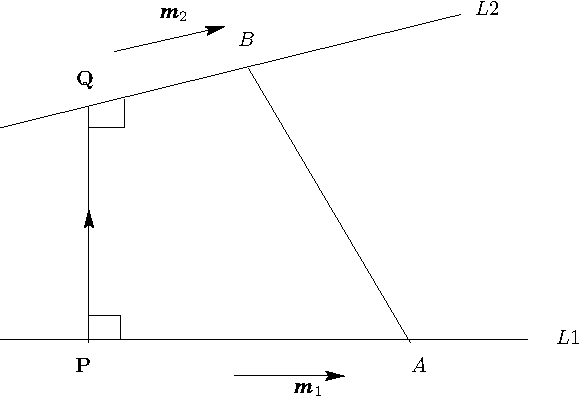
\includegraphics[width=\columnwidth]{skewlines.pdf}
	\caption{} \label{linefig1}
\end{figure}
\noindent
Since $P$ lies on $L_1$ and $Q$ lies on $L_2$, the points should satisfy 
	equations (\ref{eq1}) and (\ref{eq2}), respectively.

\noindent
%$\therefore$
\begin{align}
	\vec{PQ} = \vec{Q}-\vec{P} = \vec{B}-\vec{A} 
	                   + \myvec{\vec{m_2}-\vec{m_1}}\vec{\lambda}
\end{align}
\noindent
Since $\vec{PQ}$ is parallel to $\vec{m_1} \times \vec{m_2}$:
\begin{align}
	\vec{m_1^T}\vec{PQ} = \vec{m_1^T}\vec{(B-A)} + \vec{m_1^T}\myvec{\vec{m_2} - \vec{m_1}}\vec{\lambda}=0
\end{align}
\begin{align}
        \vec{m_2^T}\vec{PQ} = \vec{m_2^T}\vec{(B-A)} + \vec{m_2^T}\myvec{\vec{m_2} - \vec{m_1}}\vec{\lambda}=0
\end{align}

\begin{align}
	\myvec{\vec{m_1^T(m_2 - m_1)} \\ \\ \vec{m_2^T(m_2 - m_1)}}\vec{\lambda} = \myvec{\vec{m_1^T(A - B)} \\ \\ \vec{m_2^T(A - B)}}
\end{align}
The value of $\vec{\lambda}$ can be obtained from (4) and the points $\vec{P}$ and $\vec{Q}$ can be evaluated. 
%..............................................................................
\section{Solution :}
The lines intersect if :
\begin{align}
	\myvec{6\\2\\2} + \lambda_1\myvec{1\\-2\\2} = \myvec{-4\\0\\-1} + \lambda_1\myvec{3\\-2\\-2} 
\end{align}
\begin{align}
	\implies
	\lambda_1\myvec{1\\-2\\2} - \lambda_2\myvec{3\\-2\\-2} = \myvec{-4\\0\\-1} - \myvec{6\\2\\2}
\end{align}
\begin{align}
        \implies
	\myvec{1 & -3\\-2 & 2\\2 & 2}\myvec{\lambda_1 \\ \lambda_2} = \myvec{-10\\-2\\-3}
\end{align}
Row reducing the augmented matrix,
\begin{align}
	\myvec{1  & -3 & -10 \\ -2 & 2 & -2 \\ 2 & 2 & -3} 
	\xleftrightarrow[R_2 \leftarrow R_2+2R_1]{R_3 \leftarrow R_3-2R_1}
	\myvec{1  & -3 & -10 \\ 0 & -4 & -22 \\ 0 & 8 & 17}  \\
	\xleftrightarrow[]{R_3 \leftarrow R_3+2R_2}
	\myvec{1  & -3 & -10 \\ 0 & -4 & -22 \\ 0 & 0 & -23} 
\end{align}
\\
Since the above matrix has rank =3 the lines do not intersect. The direction vector of the lines are also not same and hence not parallel. Therfore the lines lie in a different plane. Such lines are known as skew lines. \\
From equation (3) we have 
\begin{align}
	\vec{PQ} = \vec{Q - P} = \myvec{-10\\-2\\-3} + \myvec{3 & -1 \\ -2 & 2 \\ -2 & -2}\vec{\lambda}
\end{align}
From equation (4):
\begin{align}
	\myvec{3 & -9 \\ 17 & -3}\vec{\lambda} = \myvec{12\\20}
	\implies
	\vec{\lambda} = \myvec{1\\-1}
\end{align}
Substituting the values in equation to obtain:
\begin{align*}
	\vec{P} = \myvec{7\\0\\4}
\end{align*}
and
\begin{align*}
	\vec{Q} = \myvec{-7\\2\\1}
\end{align*}
\begin{figure}[htbp]
\centering
	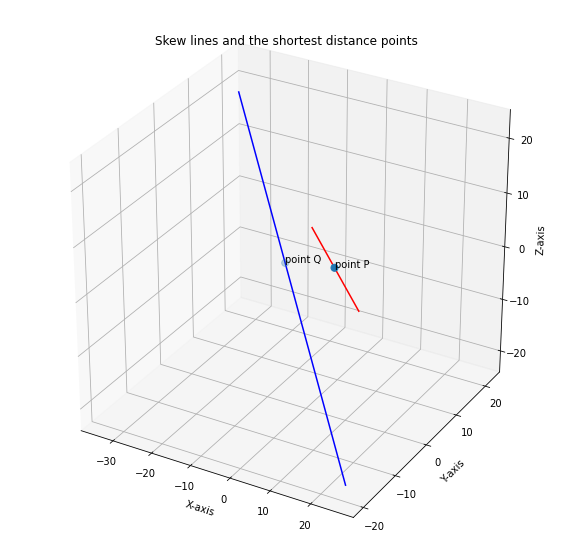
\includegraphics[width=\columnwidth]{skew_lines_plot.png}
	\caption{}
\end{figure}
%................................................................................
\end{document}
